\chapter{Appendix}
\section*{Derivation: Change of Energy per Area over Time}\label{sec:derivation:dE_dt}
For this derivation we use the non-hydrostatic NSE derived in Section~\ref{sec:non_hydrostatic}.
We also assume that $s_{top}$ and $s_{bottom}$ are constant.\\
\begin{align*}
\frac{\partial E'}{\partial t} &= \frac{\partial}{\partial t}\int_{s_{top}}^{s_{bottom}} \frac{1}{g}(C_vT+\frac{1}{2}w^2 + gz(s)) \left( \frac{\partial \pi}{\partial s} \right) ds\\
&=~~~~\int_{s_{top}}^{s_{bottom}} \frac{1}{g}\left(C_v\frac{\partial T}{\partial t}+\frac{1}{2}\frac{\partial w^2}{\partial t} + g\frac{\partial z(s)}{\partial t}\right) \left( \frac{\partial \pi}{\partial s} \right) ds \\&~~~~+ \int_{s_{top}}^{s_{bottom}} \frac{1}{g}(C_vT+\frac{1}{2}w^2 + gz(s)) \left( \frac{\partial}{\partial t}\frac{\partial \pi}{\partial s} \right) ds\\
&= \int_{s_{top}}^{s_{bottom}} \frac{1}{g}\left(C_v\frac{\partial T}{\partial t}+w\frac{\partial w}{\partial t} + g\frac{\partial z(s)}{\partial t}\right) \left( \frac{\partial \pi}{\partial s} \right) ds\\
&= \int_{s_{top}}^{s_{bottom}} \frac{1}{g}\left(\frac{C_vRT}{C_p}\frac{\partial \text{ln}p}{\partial t}-gw\left(1 - \frac{\partial p}{\partial s}\left(\frac{\partial \pi}{\partial s}\right)^{-1}\right) + g\frac{\partial}{\partial t}\left(\frac{R}{g}\int _s ^{s_{bottom}} \frac{T}{p}\left(\frac{\partial \pi}{\partial s}\right)ds'\right)\right) \\&~~~~~~~~~~~~~~~~\cdot\left( \frac{\partial \pi}{\partial s} \right) ds\\
\end{align*}
In order to enhance readability, the three terms are now transformed separately, starting with the first term (with $C_v=C_p-R$).
\begin{align*}
\frac{C_vRT}{C_p}\frac{\partial \text{ln}p}{\partial t} &= \frac{(C_p-R)RT}{C_p}\frac{g}{1- \frac{R}{C_p}} \frac{p}{RT}\left(\frac{\partial \pi}{\partial s}\right)^{-1} \frac{\partial w}{\partial s}\\
&= gp\left(\frac{\partial \pi}{\partial s}\right)^{-1} \frac{\partial w}{\partial s}
\end{align*}
For now, the second term can stay as is.
We reshape the third term as follows (assuming $w(s_{bottom})=0$):
\begin{align*}
g\frac{\partial}{\partial t}\left(\frac{R}{g}\int _s ^{s_{bottom}} \frac{T}{p}\left(\frac{\partial \pi}{\partial s}\right)ds'\right) &= R\int _s ^{s_{bottom}} \left(\frac{\partial \pi}{\partial s}\right)\frac{\partial}{\partial t}\left(\frac{T}{p}\right)ds' + R\int _s ^{s_{bottom}} \frac{T}{p}\left(\frac{\partial}{\partial t}\frac{\partial \pi}{\partial s}\right)ds'\\
&= R\int _s ^{s_{bottom}} \left(\frac{\partial \pi}{\partial s}\right)\frac{\partial}{\partial t}\left(\frac{T}{p}\right)ds'\\
&= R\int _s ^{s_{bottom}} \left(\frac{\partial \pi}{\partial s}\right)\left(-\frac{g}{R}\left(\frac{\partial\pi}{\partial s}\right)^{-1}\frac{\partial w}{\partial s}\right)ds'\\
&= -g\int _s ^{s_{bottom}} \left(\frac{\partial w}{\partial s}\right)ds'\\
&= -g\left( w(s_{bottom}) - w(s) \right)\\
&= gw(s)
\end{align*}
With these reshaped terms, $E'$ can be written as:
\begin{align*}
\frac{\partial E'}{\partial t} &= \int_{s_{top}}^{s_{bottom}} \frac{1}{g}\left(gp\left(\frac{\partial \pi}{\partial s}\right)^{-1} \frac{\partial w}{\partial s}-gw\left(1 - \frac{\partial p}{\partial s}\left(\frac{\partial \pi}{\partial s}\right)^{-1}\right)+gw \right)\left( \frac{\partial \pi}{\partial s} \right) ds\\
&=\int_{s_{top}}^{s_{bottom}} \left(p \frac{\partial w}{\partial s}+w\frac{\partial p}{\partial s}\right) ds\\
&=\int_{s_{top}}^{s_{bottom}} \left(\frac{\partial (wp)}{\partial s}\right) ds = w(s_{bottom})p(s_{bottom})-w(s_{top})p(s_{top})
\end{align*}

%\section{Laplace Transform}\label{sec:laplace_trafo}
%The Laplace Transform $\mathcal{L}\{x(t)\}(s)$ of $x(t)$ is defined as:
%\begin{align*}
%\mathcal{L}\{x(t)\}(s)=X(s)=\int_0^\infty x(t)\exp (-st)dt
%\end{align*}
%In this context $s\in \mathrm{C}$ is a complex number, and \emph{not} a vertical coordinate.\\
%For differential equations one useful identity is the Laplace Transform of derivatives:
%\begin{align*}
%\mathcal{L} \left\{ \frac{dx}{dt}(t) \right\} &=\int_0^\infty \frac{dx}{dt}(t)\exp (-st)dt\\
%&=x(t)\exp(-st)\rvert _0^\infty + s  \int_0^\infty x(t)\exp (-st)dt\\
%&=-x(t=0) + sX(s)
%\end{align*}

%\section{Error using Charney-Phillips-Grid for Stationary Solution}\label{sec:stationary_cp_error}
%\begin{figure}[htpb]
%	\makebox[\textwidth]{ 
%  		 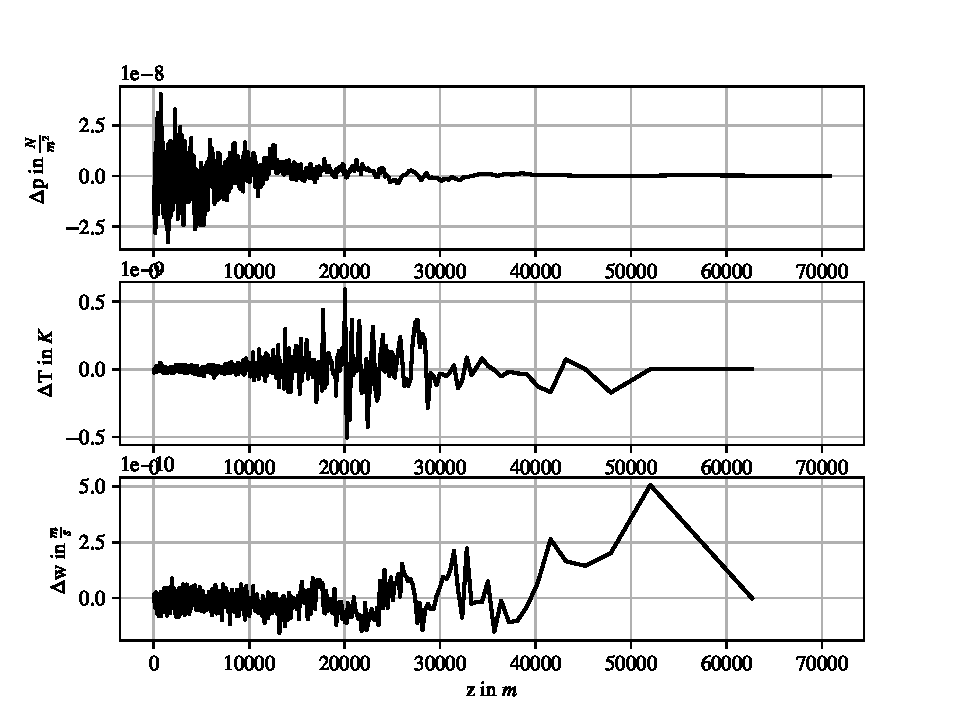
\includegraphics[width=1.0\textwidth]{figures/cp_240s_stat.pdf}}
%    \caption{Error (deviation from stationary solution) made using RK4, time-step-size $2.5ms$, and $1000$ grid points, after $240s$ of simulation time on Charney-Phillips grid}
%    \label{fig:cp_stat_err}
%\end{figure}